\documentclass[a4paper,12pt,oneside]{book}

%------------------------------- Start of the Preable ------------------------------------------------
\usepackage[english]{babel}
\addto{\captionsenglish}{%
\renewcommand{\bibname}{References}
\renewcommand{\refname}{References}
}

\usepackage{blindtext}

%\usepackage[none]{hyphenat}
\usepackage[parfill]{parskip}

\usepackage{hyperref}
\hypersetup{
    colorlinks=true,
    linkcolor=blue,
    filecolor=magenta,      
    urlcolor=cyan,
}

\urlstyle{same}
%use of package fancy header
\usepackage{fancyhdr}
\usepackage{fancyvrb}
\setlength\headheight{26pt}
\fancyhf{}
%\rhead{
\includegraphics[width=1cm]{logo}}
\lhead{\rightmark}
\rhead{
\includegraphics[width=1cm]{images/logo}}
\fancyfoot[RE, RO]{\thepage}
\fancyfoot[CE, CO]{\href{http://www.e-yantra.org}{www.e-yantra.org}}

\pagestyle{fancy}

%use of package for section title formatting
\usepackage{titlesec}
\titleformat{\chapter}
  {\Large\bfseries} % format
  {}                % label
  {0pt}             % sep
  {\huge}           % before-code
 
%use of package tcolorbox for colorful textbox
\usepackage[most]{tcolorbox}
\tcbset{colback=cyan!5!white,colframe=cyan!75!black,halign title = flush center}

\newtcolorbox{mybox}[1]{colback=cyan!5!white,
colframe=cyan!75!black,fonttitle=\bfseries,
title=\textbf{\Large{#1}}}

%use of package marginnote for notes in margin
\usepackage{marginnote}

%use of packgage watermark for pages
%\usepackage{draftwatermark}
%\SetWatermarkText{
\includegraphics{logo}}
\usepackage[scale=2,opacity=0.1,angle=0]{background}
\backgroundsetup{
contents={
\includegraphics{images/logo}}
}

%use of newcommand for keywords color
\usepackage{xcolor}
\newcommand{\keyword}[1]{\textcolor{red}{\textbf{#1}}}

%package for inserting pictures
\usepackage{graphicx}

%package for highlighting
\usepackage{color,soul}

%new command for table
\newcommand{\head}[1]{\textnormal{\textbf{#1}}}

\usepackage{dirtree}
\usepackage{siunitx}

%---------------------- End of the Preamble ---------------------------------------


\begin{document}

%---------------------Title Page------------------------------------------------
\begin{titlepage}
\raggedright
{\Large eYSIP 2017\\[1cm]}
{\Huge \scshape Control and Firmware Development for Quadcopters \\[.1in]}
\vfill
\begin{flushright}
{\large Heethesh Vhavle \\}
{\large Sanam Shakya \\}
{\large Pushkar Raj \\}
\vspace{0.5cm}
{\large Duration of Internship: $ 22/05/2017-07/07/2017 $ \\}
\end{flushright}
\medskip

{\itshape 2017, e-Yantra Publication}
\end{titlepage}

%-------------------------------------------------------------------------------

\tableofcontents
\listoffigures

%-------------------------------------------------------------------------------

\chapter[Introduction]{Introduction}
\section{Abstract}
The project deals with the study of control algorithms and to develop a custom firmware for quadcopter (flight controller) on 32-bit micro-controllers such as the STM32F1xx (ARM® Cortex®-M3 core). The flight controller is designed to control parameters such as the throttle, yaw, pitch and roll and consists of algorithms considering various motion and dynamics. The next step is to analyze the control algorithm to identify effects of various parameters and to optimize it for stable motion. The final step is to develop a wireless joystick controller for simple maneuvering of the quadcopter. 

\section{Completion Status}
\begin{enumerate}
\item Flight controller firmware development is complete. Various libraries such as UART, I2C, Timers, PWM, various sensors, MSP, motors, joystick and PID control libraries were developed for the firmware.

\item Sensor interfacing is complete. The MPU9250 IMU (Accelerometer and Gyroscope) and AK8963 Magnetometer were successfully interfaced, calibrated and the filtered pitch, roll and yaw angles were obtained. The MS5611 Barometer was successfully interfaced as well and an estimate of altitude, based on the pressure readings, was obtained.

\item The MultiWii Serial Protocol (MSP) was implemented for communication with the flight controller and for telemetry purposes. Real time data can be visualized using Python or MultiWii Conf.

\item An USB joystick controller was interfaced with the PC and using Python, wireless control of the quadcopter was developed.

\item A control architecture was designed for pitch, roll, yaw and throttle  control, with a PID controller implemented for each axis. On-the-fly PID tuning was implemented along with a GUI developed for the same. The PID gains for the pitch, roll and yaw axes were tuned. However, fine tuning of these gains are not yet complete.

\item Quadcopter flight was achieved and parameters such as pitch, roll, yaw, throttle and trim were successfully controlled using the joystick controller. However, the flight is not stable yet and the quadcopter experiences drift in motion. Altitude hold feature is yet to be implemented.\\
\end{enumerate}

\begin{figure}[!htb]
\centering
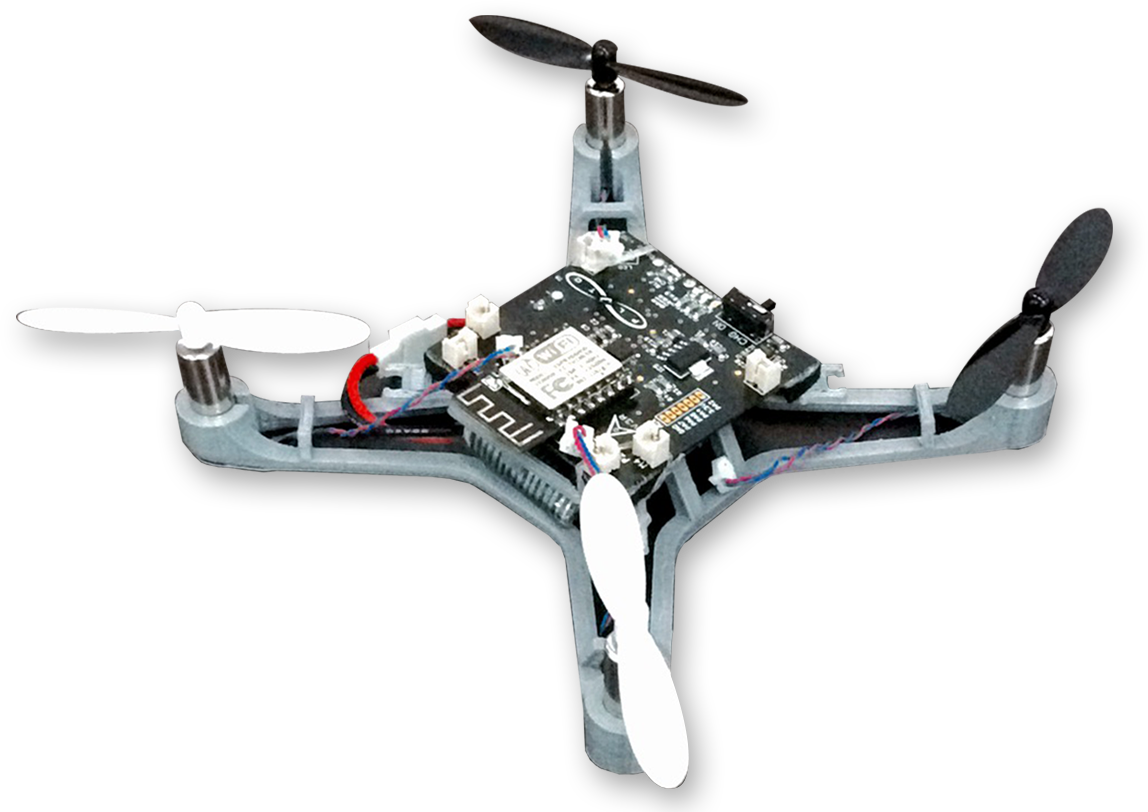
\includegraphics[width=0.8\textwidth]{images/pluto_drone}
\caption{Pluto Drone by Drone Aviation}
\end{figure}

%-------------------------------------------------------------------------------

\chapter[Hardware]{Hardware}
One of the goals of the project is to develop a firmware for 32-bit micro-controllers. The micro-controller used in this project is the STM32F103 (ARM Cortex-M3 Core). Initially the firmware development was carried out on the Nucleo Development Board. The quadcopter, used in the later stage, is the Pluto Drone, provided by Drona Aviation. The following section lists all the hardware components used in this project along with its specifications.

\section{List of Hardware Components}
\begin{itemize}
\item NUCLEO-F103RB STM32 Nucleo Development Board \\
\href{./datasheets/Nucleo STM32 Board.pdf}{Datasheet} | \href{./datasheets/STM32F103X.pdf}{Chip Datasheet} | \href{http://in.element14.com/stmicroelectronics/nucleo-f103rb/nucleo-board-stm32f103rbt6-mcu/dp/2394226}{Vendor Link}

\item Drona Aviation - Pluto Drone \\
\href{./datasheets/Pluto Drone Schematic.pdf}{Schematic} | \href{http://www.dronaaviation.com/}{Vendor Link}

\begin{itemize}
\item STM32F103C8 Micro-controller\\
\href{./datasheets/STM32F103X.pdf}{Datasheet} | \href{./datasheets/STM32F1 Reference Manual.pdf}{Reference Manual} | \href{./datasheets/Geoffrey Brown - Discovering the STM32 Microcontroller.pdf}{Guide Book} | \href{http://www.amazon.in/STM32F103C8T6-Minimum-System-Development-Arduino/dp/B01EM11KOC/ref=sr_1_1?ie=UTF8&qid=1499069205&sr=8-1&keywords=STM32F103C8T6}{Vendor Link}

\item MPU9250 Accelerometer and Gyroscope \\
\href{./datasheets/MPU9250 Datasheet.pdf}{Datasheet} | \href{./datasheets/MPU9250 Register Map.pdf}{Register Map} | \href{http://www.amazon.in/Generic-MPU-9250-Communications-gyroscope-accelerometer/dp/B06XPLH7KD/ref=sr_1_2?ie=UTF8&qid=1499068377&sr=8-2&keywords=mpu9250}{Vendor Link}

\item AK8963 Magnetometer \\
\href{./datasheets/AK8963.pdf}{Datasheet} | \href{http://www.amazon.in/Generic-MPU-9250-Communications-gyroscope-accelerometer/dp/B06XPLH7KD/ref=sr_1_2?ie=UTF8&qid=1499068377&sr=8-2&keywords=mpu9250}{Vendor Link}

\item MS5611 Barometer\\
\href{./datasheets/MS5611-01BA03.pdf}{Datasheet} | \href{http://www.amazon.in/MS5611-High-Resolution-Atmospheric-Pressure-Arduino/dp/B00ZA7DMGC/ref=sr_1_3?ie=UTF8&qid=1499068488&sr=8-3&keywords=ms5611}{Vendor Link}

\item ESP8266 Wi-Fi Wireless Module\\
\href{./datasheets/ESP8266-Datasheet.pdf}{Datasheet} | \href{http://www.amazon.in/ESP8266-Serial-Wireless-Arduino-Raspberry/dp/B00TS5TMRK/ref=sr_1_3?ie=UTF8&qid=1499068563&sr=8-3&keywords=ESP8266}{Vendor Link}

\item Coreless Motors and Propellers \\
\href{http://www.amazon.in/Engineerstoys-Coreless-Motor-Propeller-Set/dp/B01HTIN6CE/ref=sr_1_2?ie=UTF8&qid=1499068914&sr=8-2&keywords=coreless+motor}{Vendor Link}

\item 3.7V Li-Po Battery \\
\href{http://www.amazon.in/Generic-Cheerson-Quadcopter-Ariplane-shipping/dp/B071XYV3HR/ref=sr_1_8?ie=UTF8&qid=1499068765&sr=8-8&keywords=3.7v+lipo}{Vendor Link}

\end{itemize}
\end{itemize}

\section{STM32 Micro-controller}
The STM32 family of micro-controllers, based upon the ARM Cortex-M3 core, provides a foundation for building a vast range of embedded systems from simple battery powered dongles to complex real-time systems such as helicopter autopilots. This component family provides wide-ranging choices in memory sizes, available peripherals, performance, and power. Unfortunately, power and flexibility are achieved at a cost – software development for the STM32 family can be extremely challenging for the uninitiated with a vast array of documentation and software libraries to wade through.\cite{geob} \\

The STM32F103xx medium-density performance line family incorporates the high-performance ARM Cortex-M3 32-bit RISC core operating at a 72 MHz frequency, high-speed embedded memories (Flash memory up to 128 Kbytes and SRAM up to 20 Kbytes), and an extensive range of enhanced I/Os and peripherals connected to two APB buses. All devices offer two 12-bit ADCs, three general purpose 16-bit timers plus one PWM timer, as well as standard and advanced communication interfaces: up to two I2Cs and SPIs, three USARTs, an USB and a CAN.\cite{stm32}

\begin{figure}[!htb]
\centering
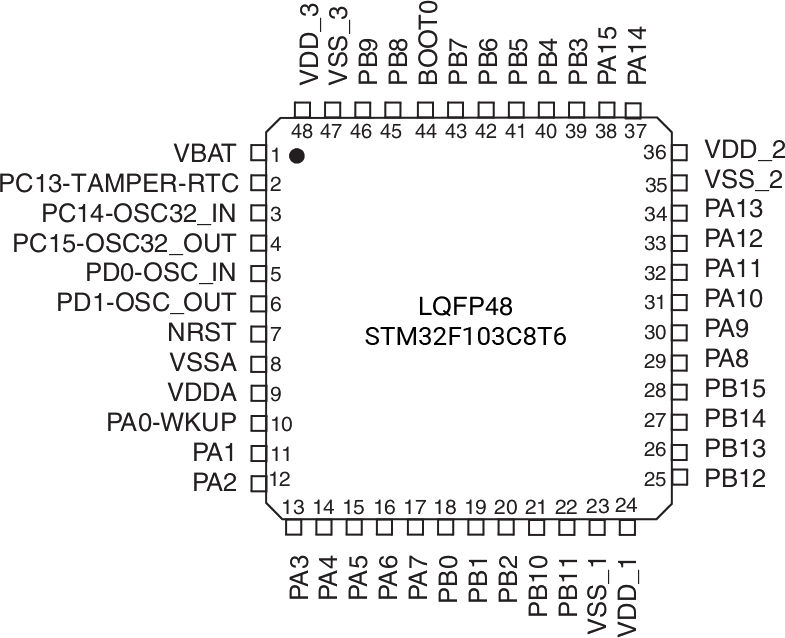
\includegraphics[width=0.6\textwidth]{images/stm32_pinout}
\caption{Pinout diagram of STM32F103C8T6 LQFP48 package}
\end{figure}

\section{Hardware Schematic}
The Pluto Drone embedded board consists of the STM32F103C8 micro-controller. MPU9250 IMU and MS5611 Barometer are interfaced on I2C1 bus. The AK8963 Magnetometer is interfaced as a slave device to the MPU9250 master (refer to Section 3.1.1 for further details). Although the board supports upto six motor connections, only four are used (M1-M4), which are connected to the PWM channel pins. VL53L0X is a LASER ranging sensor, which is currently not interfaced. There are three on-board indicator LEDs (D1, D2 and D3). \textit{\autoref{fig:schematic}} shows the hardware schematic.

\begin{figure}[!htb]
\centering
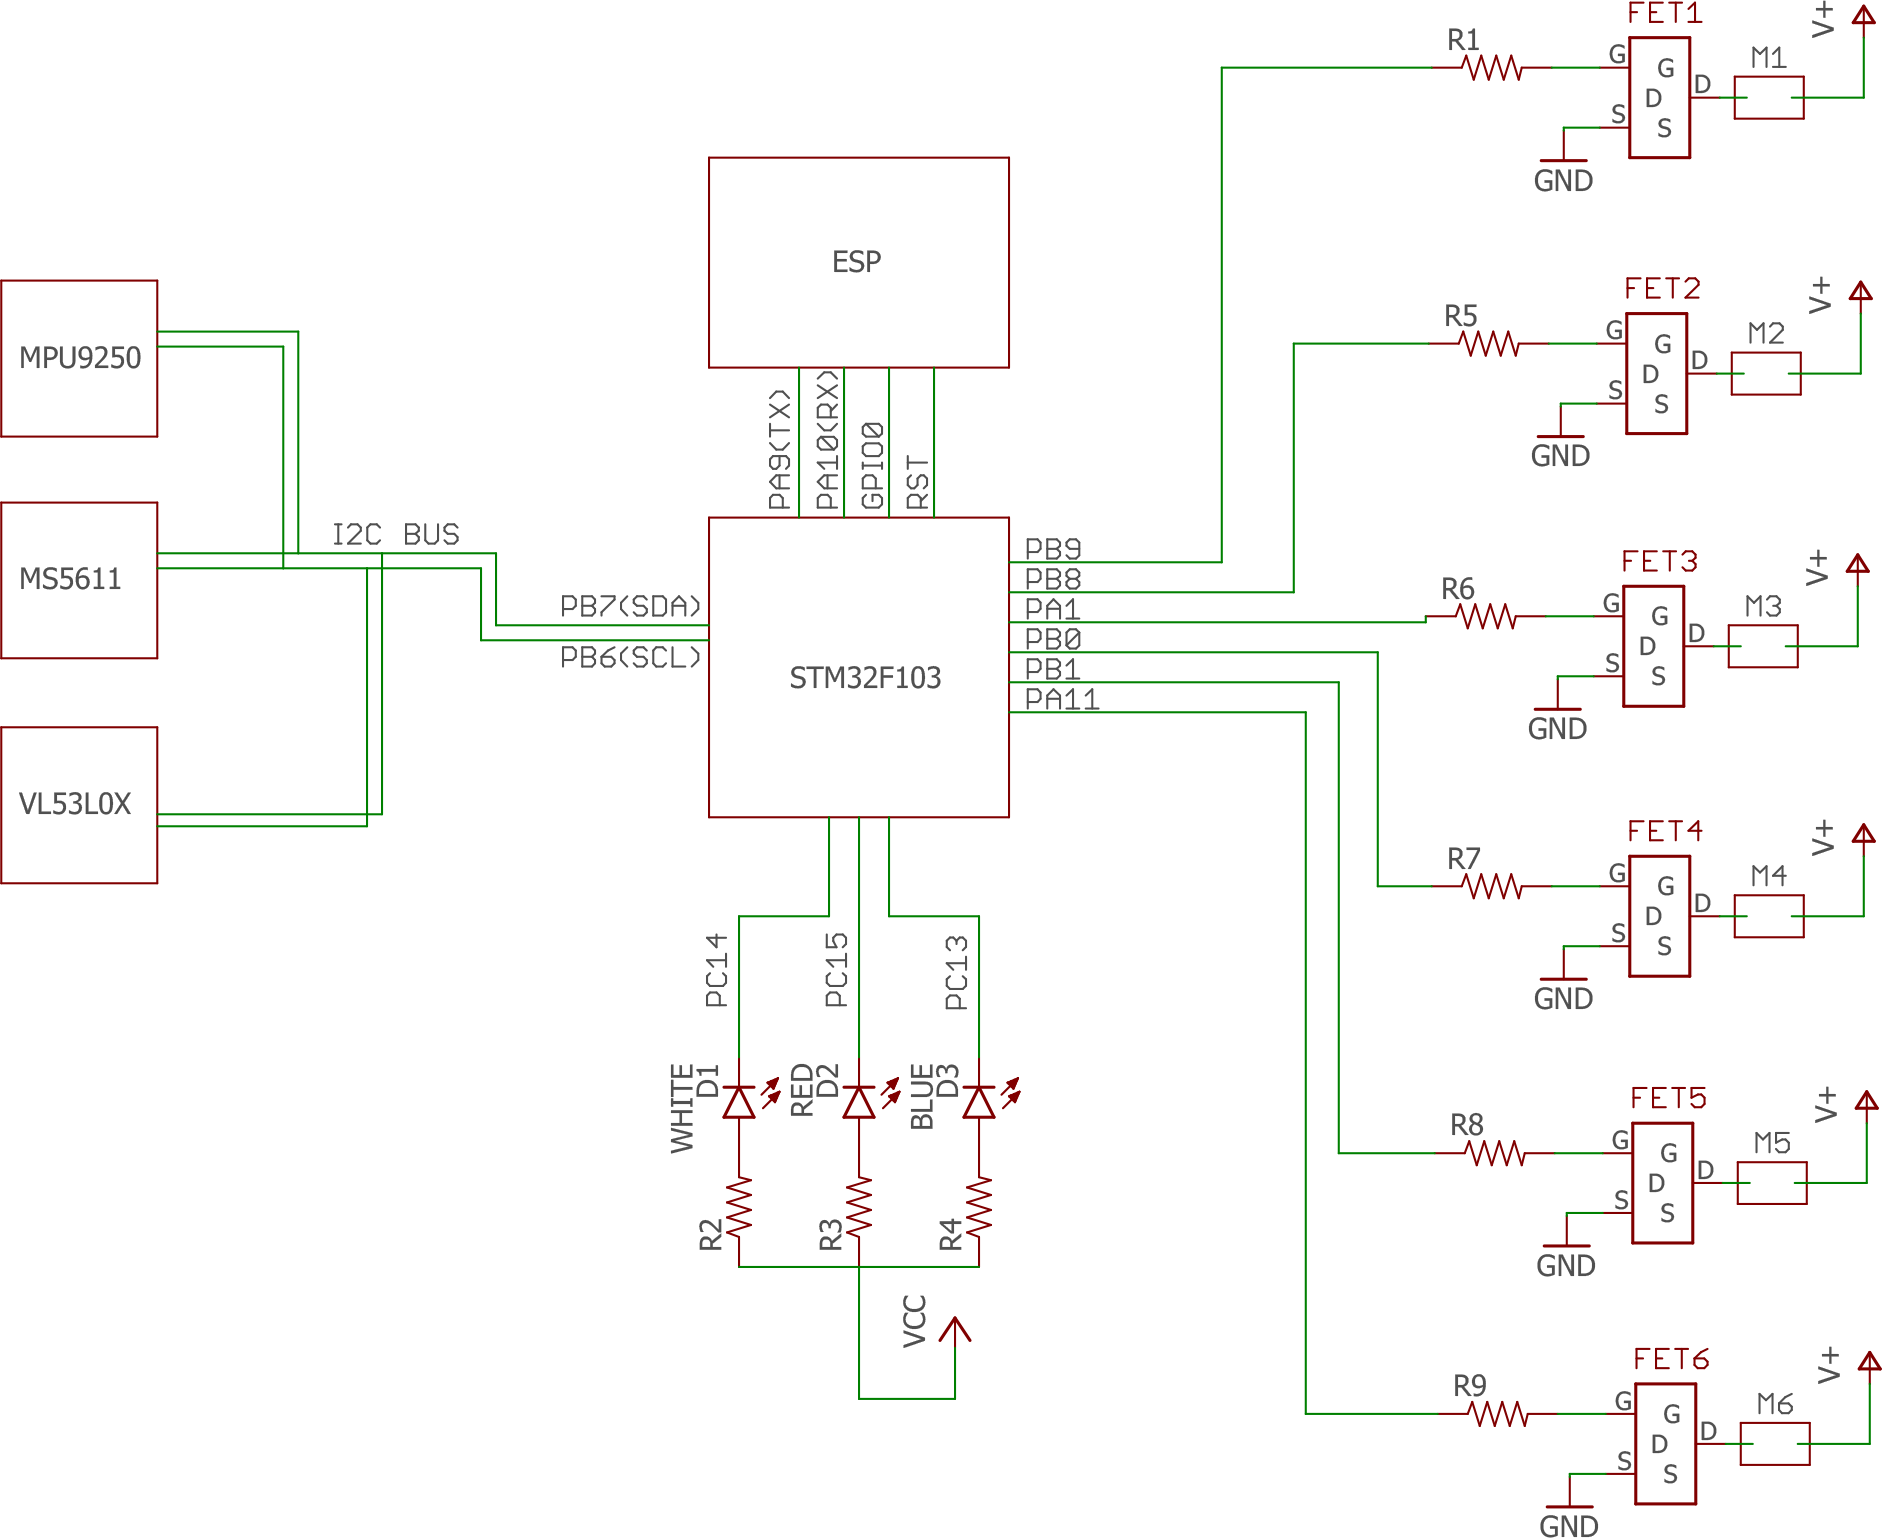
\includegraphics[width=\textwidth]{images/pluto_drone_schematic}
\caption{Hardware schematic of Pluto Drone}
\label{fig:schematic}
\end{figure}

\chapter[Software]{Software}
The primary software resource is the GNU software development tool-chain including gcc, objcopy, objdump, and the debugger gdb. The GNU ARM Embedded tool-chains are integrated and validated packages featuring the ARM Embedded GCC compiler, libraries and other GNU tools necessary for bare-metal software development on devices based on the ARM Cortex-M and Cortex-R processors.\cite{geob, gnu} The entire firmware is written in C language. Coming to IDE, various different options are available such as ARM Keil MDK, EWARM, TrueSTUDIO and open source options such as the Eclipse IDE.

\section{Installation of Softwares and Tools}
This section gives a brief overview on setting up the IDE and the various methods of flashing the program on to the micro-controller.

\subsection{Integrated Development Environment (IDE)}
The Eclipse IDE requires the tool-chain, debug and build tools to be installed manually. The tool-chains are available for cross-compilation on Microsoft Windows, Linux and Mac OS X host operating systems. The tool-chain can be downloaded from \href{https://launchpad.net/gcc-arm-embedded/}{here}.\cite{gnu}\\

The IDE used is in this project is \href{https://atollic.com/resources/download/}{Attolic TrueSTUDIO}, which is based on the Eclipse IDE. One of the main advantages is that TrueSTUDIO IDE already comes with the GCC tool-chains for ARM and the required debugging tools.\\ 

\subsection{Debugging Tools}
One of the key feature of Nucleo board is that it already provides the on-chip programmer for STM32 micro-controllers. In order to use this, \href{http://www.st.com/en/embedded-software/stsw-link009.html}{ST-LINK drivers} need to be installed.\\

Although TrueSTUDIO has built-in debugging tools, some of the features are not available in the free version of the software. Instead, we can use the official \href{http://www.st.com/en/embedded-software/stsw-link004.html}{ST-LINK Utility} tool.\\

\subsection{Flashing the Program}
There are three ways to upload the firmware on to the micro-controller. One of the easiest way is to simply generate a \textit{binary (*.bin)} file, connect your board via USB and it should be detected as an external storage device. Program can be flashed by just dragging and dropping the binary file on the device.\\

The ST-LINK Utility tool also supports flashing the program on to the board. One can alternatively use the \href{http://www.amazon.in/xcluma-St-Link-Stlink-Emulator-Downloader/dp/B072TFSGW7/ref=sr_1_1?ie=UTF8&qid=1499104526&sr=8-1&keywords=st+link}{ST Link V2 Programmer}. The header for this programmer contains connections for 5V, 3.3V, SWCLK, SWDIO, SWIM, Reset (RST/NRST) and GND. The connector on the opposite side of this device is a USB connector and is intended to be plugged into the computer for programming.\\

Another method of flashing the program is by using the built-in UART Bootloader. Further details are explained \href{http://www.scienceprog.com/flashing-programs-to-stm32-embedded-bootloader/}{here}. An USART to USB driver chip like FT232 can be used along with \href{http://www.st.com/en/development-tools/flasher-stm32.html}{STM32 Flash Loader Demonstrator} to flash the program. The \textit{Pluto Drone} board supports wireless programming (UART Bootloading) with the help of the ESP8266 which is connected to the boot, reset and USART pins on the board. \href{https://chrome.google.com/webstore/detail/cleanflight-configurator/enacoimjcgeinfnnnpajinjgmkahmfgb?hl=en}{CleanFlight Configurator} software can be used to flash the program (\textit{*.hex}) over Wi-Fi. 

\section{Programming the STM32 Micro-controller}

Programming the STM32 series micro-controllers is done in various layers namely, CMSIS, HAL, BSP and Application code. The software stack is shown in \textit{\autoref{fig:software_stack}}.\\

The \textit{Cortex Micro-controller Software Interface Standard (CMSIS)} supports developers in creating reusable software components for ARM Cortex-M based systems. It mostly contains definitions for the various registers.\\

The \textit{Hardware Abstraction Layer (HAL)} drivers were designed to offer a rich set of APIs and to interact easily with the application upper layers. Each driver consists of a set of functions covering the most common peripheral features such as GPIO, UART, I2C, CAN and so on.\cite{stm32hal}\\

When a STM32 micro-controller starts, it needs an hardware configuration to work correctly. Unfortunately, the development of one's own HAL requires a deep knowledge of the specific micro-controller. ST provides a dedicated tool that generates the initialization code and provides us the HAL peripheral drivers. This tool is called \href{http://www.st.com/en/development-tools/stm32cubemx.html}{STM32CubeMX} and it is very useful.\cite{carmine}\\

\begin{figure}[!htb]
\centering
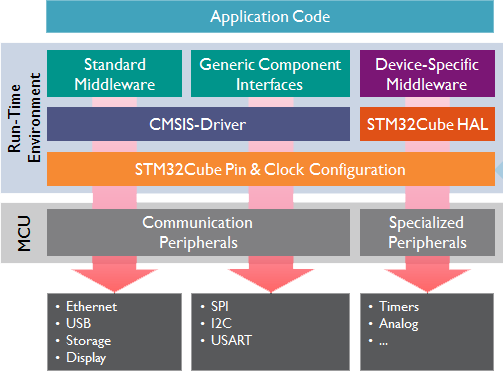
\includegraphics[width=0.7\textwidth]{images/software_stack}
\caption{Software stack for STM32 programming}
\label{fig:software_stack}
\end{figure}

\chapter[Flight Controller Firmware]{Flight Controller Firmware}
The motivation behind developing a custom flight controller firmware from scratch is that one can optimize the flight performance up to middleware layer. It may seem like a lot of effort to be put in to develop such a firmware from scratch initially, but once it is developed it is more advantageous to the user than using an already existing flight controller. Some advantages are that it allows for great customization and flexibility in terms of the control algorithm and in optimizing the flight dynamics, implementing our own communication and telemetry protocols for specific usage and allows for more advanced pilot control and features to be implemented easily.\\

Although open-source flight controllers like \textit{CleanFlight} and \textit{dRonin} exist, it is limited in terms of the customization aspect as these are designed to support a vast array of hardwares. Making a simple modification to a certain feature requires one to wade through the vast amount of libraries and requires good knowledge about the firmware implementation.\\

\section{Structural Overview}
A brief overview of the software stack was given in the previous chapter. The two most common peripheral drivers available for STM32 micro-controllers are \textit{Standard Peripheral Library} and \textit{STM32Cube HAL}. The later is used in the firmware as it is a  more standardized method and is less error-prone as the driver initialization code is auto generated.\\

Firmware development in this project began from the \textit{Board Specific Package (BSP)} layer with development of libraries such as GPIO, I2C, Serial, Timing and PWM. Once these libraries were ready, the application layer development began with libraries for the different sensor, filters, control algorithms, telemetry protocols (MSP) and joystick interfacing. \textit{\autoref{fig:folders}} shows the basic directory  structure of the firmware. \textit{Note: Only  header files are shown}.\\

\begin{figure}[!htb]
\centering
\framebox[\textwidth]{%
\begin{minipage}{0.5\textwidth}
\dirtree{%
.1 firmware/.
	.2 Drivers/.
		.3 CMSIS/.
		.3 STM32F1xx{\_}HAL{\_}Driver/.
			.4 stm32f1xx{\_}hal.h.
			.4 stm32f1xx{\_}hal{\_}gpio.h.
			.4 stm32f1xx{\_}hal{\_}uart.h.
			.4 \vdots.
	.2 Include/.
		.3 circular{\_}buffer.h.
		.3 common.h.
		.3 devices.h.
		.3 i2c.h.
		.3 joystick.h.
		.3 MadgwickAHRS.h.
		.3 motor.h.
		.3 MPU9250.h.
		.3 MS5611.h.
		.3 msp.h.
		.3 peripherals.h.
		.3 pid.h.
		.3 serial.h.
		.3 timing.h.
	.2 Source/.
		.3 main.c.
		.3 stm32f1x{\_}it.c.
		.3 \vdots.
	.2 Debug/.
		.3 firmware.hex.
		.3 firmware.bin.
		.3 \vdots.
}
\end{minipage}
}
\caption{Directory structure of the flight controller firmware}
\label{fig:folders}
\end{figure}

\section{Board Specific Package (BSP)}
The BSP layer bridges the gap between the device drivers and the application layer. While the HAL only provides the peripheral initialization, the BSP implements the functionality of the peripherals which is used by the application layer. In the current firmware, the following libraries are a part of the BSP.\\

\begin{enumerate}
\item  \textbf{peripherals.h} | This library consists of all the HAL peripheral initialization code and provides a master \textit{Devices{\_}Init()} function. It also handles the system clock configuration and error handling function.\\

\item \textbf{devices.h} | This library handles all of the I/O interfacing such as LED control and PWM write functions.\\

\item \textbf{timing.h} | The timing library provides the \textit{delay{\_}ms()} and \textit{millis()} functions, built using \textit{SysTick}.\\

\item \textbf{serial.h} | The serial library consists of serial read and write functions for a single byte from the circular buffer. The UART interrupt callback functions of the HAL are implemented in this library. It also provides functions for printing strings, floats and integers on a terminal.\\

\item \textbf{circular{\_}buffer.h} | A circular buffer is required to store the received data when using interrupts for UART communication. Further details of UART communication is explained in \autoref{sec:comm}.\\

\item \textbf{i2c.h} | This library provides function to write a single byte and read individual as well as multiple bytes over I2C protocol.\\

\item \textbf{common.h} | This library consists of all the miscellaneous functions such as \textit{map()}, \textit{map{\_}float()}, \textit{constrain()} and \textit{lowPassFilter()} and is used by higher level libraries.\\

\end{enumerate}

\section{Attitude and Heading Reference System}

One of the most trivial and important tasks of a flight controller firmware is control and stabilization of the orientation of the quadcopter. The three axes of orientation involved are namely pitch, roll and yaw as shown in \autoref{fig:AHRS}\\

An \textit{Attitude and Heading Reference System (AHRS)} consists of sensors on three axes that provide attitude information for aircraft, including roll, pitch and yaw. They are designed to replace traditional mechanical gyroscopic flight instruments and provide superior reliability and accuracy.\cite{ahrswiki}\\

AHRS consist of either solid-state or microelectromechanical systems (MEMS) gyroscopes, accelerometers and magnetometers on all three axes. A form of non-linear estimation such as an Extended Kalman filter is typically used to compute the solution from these multiple sources. One abbreviation used in technology for sensor arrays used in AHRS is MARG (Magnetic, Angular Rate, and Gravity).\cite{ahrswiki}\\

\begin{figure}[!htb]
\centering
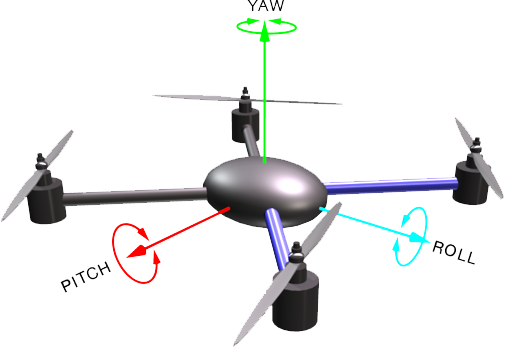
\includegraphics[width=0.7\textwidth]{images/AHRS}
\caption{The pitch, roll and yaw angles (AHRS) of a quadcopter\cite{ardu}}
\label{fig:AHRS}
\end{figure}

\subsection{MPU9250 Accelerometer and Gyroscope}
The \href{./datasheets/MPU9250 Datasheet.pdf}{MPU-9250} is an inertial measurement unit (IMU). MPU-9250 features three 16-bit analog-to-digital converters (ADCs) for digitizing the gyroscope outputs, three 16-bit ADCs for digitizing the accelerometer outputs, and three 16-bit ADCs for digitizing the magnetometer outputs. For precision tracking of both fast and slow motions, the parts feature a user-programmable gyroscope full-scale range of $\pm$250, $\pm$500, $\pm$1000, and $\pm$\SI{42}{\degree\per\second} (dps), a user-programmable accelerometer full-scale range of $\pm$2g, $\pm$4g, $\pm$8g, and $\pm$16g, and a magnetometer full-scale range of $\pm$4800$\mu$T. The MPU-9250 can be interfaced via SPI or I2C. In our case, I2C at \SI{400}{\kilo\hertz} is used to interface the sensor.\\

\begin{figure}[!htb]
\centering
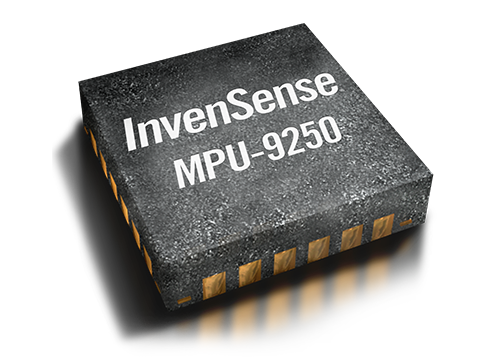
\includegraphics[width=0.4\textwidth]{images/mpu-9250}
\caption{InvenSense MPU-9250 QFN package\cite{mpu9250}}
\end{figure}

Accelerometers are devices that measure static acceleration in all the three axes. They measure in G-forces (g) equivalent to \SI{9.8}{\kilo\gram\meter\per\second\squared}. Most accelerometers will have a selectable range of forces they can measure. These ranges can vary from $\pm$1g up to $\pm$250g. Typically, the smaller the range, the more sensitive the readings will be from the accelerometer. In our case, the selected range is $\pm$4g.\cite{tonik}\\

Assuming no external forces act (except gravity) on the accelerometer, the pitch and roll angles can easily be computed by knowing the components of gravity in the different axis, which is the sensor output. By using trigonometric formulas, we can easily compute these angles. Practically, the accelerometer not only measures gravity but also all the other vibrations and the output is very noisy. This noise can be filtered out with the help of a gyroscope.\\

The gyroscope sensor within the MEMS is tiny (between 1 to 100 micrometers). When the gyro is rotated, a small resonating mass is shifted as the angular velocity changes. This movement is converted into very low-current electrical signals that can be amplified and read by a host micro-controller \cite{gyro}. The range of the gyroscope selected is $\pm$1000 dps.\\

\begin{figure}[!htb]
\centering
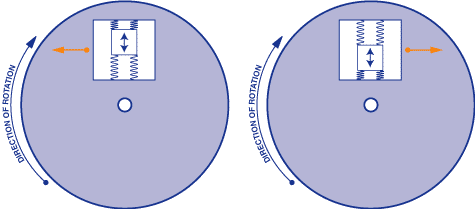
\includegraphics[width=0.7\textwidth]{images/gyro_mems}
\caption{Internal operational view of a MEMS gyro sensor\cite{gyro}}
\end{figure}

However, the gyroscope output doesn't give the angular orientation. It gives the angular rate of orientation around the three axes. This rate has to be integrated over time in order to obtain the orientation angles. But the main disadvantage of the gyroscope is that its value drifts over time due to rounding off errors and keeps accumulating these errors as we integrate it.\\

One of the solutions to combat this problem is to fuse the sensor data from both the accelerometer and the gyroscope. A simple filter like a complimentary filter can be used to achieve this. The result of this filter is pretty good. The accelerometer provides gravity as an absolute reference and helps to correct the drift from of the gyroscope.\\ 

However, this solution only provides us with only the pitch and roll angles. We also require to know the heading of the quadcopter or the yaw angle. Although, the gyroscope can measure the yaw rate of rotation, the accelerometer has no means to detect a change in yaw direction, as it only refers to gravity. Without a reference in the yaw direction, the gyroscope output will again drift. Now, that's where the Magnetometer comes in to provide this absolute reference.\\

\subsection{AK8963 Magnetometer}
The AK8963 Magnetometer is 3-axis electronic compass IC with high sensitive Hall sensor technology. This sensor is interfaced as an auxiliary sensor to the MPU-9250. The MPU-9250 acts as a master to any external sensors connected to the auxiliary I2C bus. To access the magnetometer via MPU-9250, the \textit{BYPAS{\_}EN} bit in the \textit{INT Pin / Bypass Enable Configuration} register of the MPU-9250 has to be set. Further details about this can be found in  \href[page=23]{./datasheets/MPU9250 Datasheet.pdf}{Page 23 - Datasheet}.\\

Magnetometers are wonderful devices and absolutely essential for correcting gyro drift in applications that require absolute orientation through sensor fusion. The bane of magnetometer usage is, however, their non-ideal response surfaces. The ideal response surface for a three-axis magnetometer is a sphere centered at the 3D origin. This means the response to an external magnetic field of, let's say 400 milliGauss (mG) in the z-direction would be exactly Mz = 400 mG when the magnetometers z-axis was normal to the floor, My = 400 mG when the magnetometer's y-axis was normal to the floor, and Mx = 400 mG when the magnetometer's x-axis was normal to the floor. More simply, the ideal response surface no matter the orientation of the magnetometer is a sphere with radius 400 mG centered on the origin. In practice, MEMS magnetometers are rarely so well calibrated when you receive them. There are good reasons for this. The MEMS sensors are typically characterized at the factory but mounting on a PC board can add stresses that can easily result in a shift of the calibration.\cite{kris}\\

There is an additional common type of magnetometer bias often encountered which is due to the presence of man-made sources of magnetic field like big steel buildings and current carrying wires, etc. Encounters with these environmental sources of magnetic field can be interpreted as changes in orientation if a magnetic anomaly algorithm is not employed to detect and prevent it.\cite{kris}\\

\begin{figure}[!htb]
\centering
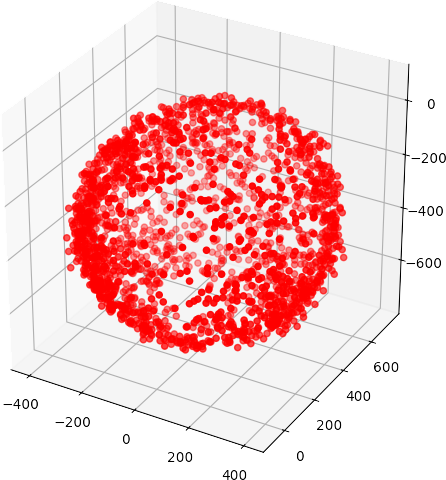
\includegraphics[width=0.7\textwidth]{images/raw}
\caption{Magnetic field in mG along X, Y and Z axes measured for an uncalibrated sensor}
\label{fig:magraw}
\end{figure}

The data plotted in \textit{\autoref{fig:magraw}} was taken by slowly turning the sensor board through a variety of figure-eight patterns. The data is properly-scaled (mG) Mx, My, and Mz values plotted using \textit{Matplotlib} in Python. Following are the observations that can be inferred from the uncalibrated sensor data.\\

\begin{enumerate}
\item The response between axes is not centered at the origin.
\item The response sensitivity is different along each axis. 
\end{enumerate}

These are often referred to as hard iron and soft iron biases, respectively.\\

\textbf{Hard iron biases} are typically the largest and the easiest errors to correct for. The simplest way to correct for them is to record a bunch of magnetometer data as the sensor is moved slowly in a figure eight pattern and keep track of the minimum and maximum field measured in each of the six principal directions; +/- Mx, +/- My, +/- Mz. Once the min/max values along the three axes are known, the average can be subtracted from the subsequent data which amounts to re-centering the response surface on the origin \cite{kris}. \textit{\autoref{fig:magoffset}} shows the hard iron bias calibrated sensor data.\\

\begin{figure}[!htb]
\centering
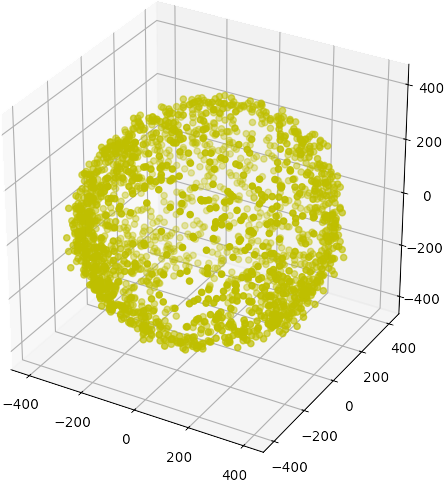
\includegraphics[width=0.57\textwidth]{images/offset}
\caption{The AK8963 magnetometer data after subtraction of the three axial offset biases}
\label{fig:magoffset}
\end{figure}

\begin{figure}[!htb]
\centering
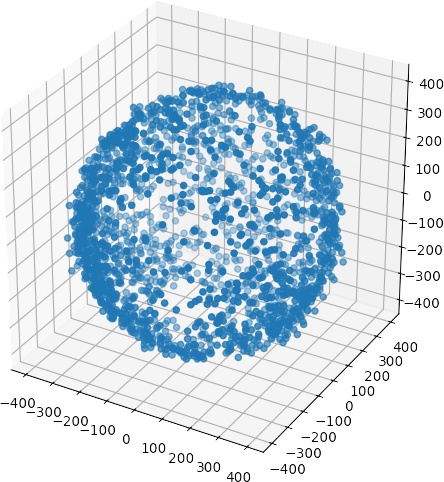
\includegraphics[width=0.57\textwidth]{images/scaled}
\caption{The MPU9250 magnetometer response after offset and scaling bias corrections}
\label{fig:magscale}
\end{figure}

\clearpage
\textbf{Soft iron bias} correction is re-scaling the axial response to make is even more spherical. It means deconstructing the response surface into its elliptical principle axes and devising a 3 x 3 correction matrix to transform the general ellipsoidal response surface into a spherical one. The min/max values which are already computed are used to rescale the magnetometer data and compute a scale factor for all three axes. Finally, the calibrated sensor data is shown in \textit{\autoref{fig:magscale}}.\cite{kris}\\

\subsection{Sensor Fusion using Madgwick's AHRS Filter}
A MARG (Magnetic, Angular Rate, and Gravity) sensor is a hybrid IMU which incorporates a tri-axis magnetometer. An IMU alone can only measure an attitude (pitch and roll angles) relative to the direction of gravity which is sufficient for many applications. MARG systems, also known as AHRS (Attitude and Heading Reference Systems) are able to provide a complete measurement of orientation relative to the direction of gravity and the earth's magnetic field.\cite{madgwick}\\

The task of an orientation filter is to compute a single estimate of orientation through the optimal fusion of gyroscope, accelerometer and magnetometer measurements. The Kalman filter has become the accepted basis for the majority of orientation filter algorithms. However, implementation of these filters demand a large computational load and not very efficient for embedded systems.\cite{madgwick}\\

Madgwick's algorithm uses a quaternion representation, allowing accelerometer and magnetometer data to be used in an analytically derived and optimised gradient descent algorithm to compute the direction of the gyroscope measurement error as a quaternion derivative. The library for Madgwick's AHRS filter is available \href{http://x-io.co.uk/open-source-imu-and-ahrs-algorithms/}{here} and further details of the working of the filter can be found \href{./datasheets/Madgwick Internal Report.pdf}{here}.\cite{madgwick}\\

\section{Altitude Measurement}
Altitude can be determined based on the measurement of atmospheric pressure. The greater the altitude, the lower the pressure. When a barometer is supplied with a nonlinear calibration so as to indicate altitude, the instrument is called a pressure altimeter or barometric altimeter. It is very important to know the altitude of a flight and altitude stabilization is required for better control of the quadcopter.

\subsection{MS5611 Barometer}
The MS5611 is a barometric pressure sensor is optimized for altimeters and variometers with an altitude resolution of 10 cm. This sensor is also interfaced on the same I2C bus as that of the IMU.\\

In order to estimate the altitude, first we have to get the pressure  and temperature data from the sensor. The pressure and temperature data is obtained as 24-bit word (3 bytes) after internal ADC conversion. However, this data may not be very useful and must be calibrated and compensated before using them. The MS5611 has a 128 bit PROM where six calibration co-efficients are stored permanently. Using these co-efficients (can be read and stored on the STM32 ROM once initially), the temperature and temperature compensated pressure can be calculated. The compensation and data conversion procedure is explained in the \href[page=7]{./datasheets/MS5611-01BA03.pdf}{datasheet}.\\

Now that we have the current pressure (in millibar), by knowing the pressure at sea level (1013.25 millibar), the altitude can be estimated by using the following formula.\\

\begin{minipage}{\textwidth}
\centering
$Altitude = 44330 \times \left [1 - \left (\frac{P}{P_{0}}\right )^{\frac{1}{5.255}} \right ]$
\end{minipage}
\clearpage

\section{Communication and Telemetry}
\label{sec:comm}
Fine tuning PID values of a quadcopter flight controller can be very devious and time consuming process if a programmer needs to adjust parameters in source code, compile it and upload the new program to copter every time they want to make a slight adjustment.\\ 

In addition to transferring new PID values to quadcopter, we can also request other data from the quadcopter, such as current PID values, sensor readings, flight status, motor values and any other data useful in error handling, debugging or even visualization.\\

A trivial problem that follows this is a standard and a secure method of data transfer. There has to some method to differentiate the various data types that we require to transmit. The \textit{MultiWii Serial Protocol (MSP)} has been devised to solve this exact problem.\\

\subsection{MultiWii Serial Protocol}
\textit{MultiWii Serial Protocol} is a part of the MultiWii flight controller firmware and has gained popularity and is currently widely used as the communication protocol in many flight controllers. It is a standard, secure and light weight protocol. MSP operates over UART communication. The data to be sent or received is packed into a frame. Each frame has a header, data payload and a checksum. The frame format is explained in detail below.\\

\textbf{Header} | Every frame begins with the characters \textit{'\$'} followed \textit{'M'}. The next element represents the direction of the data transfer. '$\langle$' indicates that the data is being sent to the quadcopter and '$\rangle$' indicates that the data is being sent from the quadcopter to a PC for telemetry or other purposes. To differentiate different types of data frames being sent (like sensor data, PID values and so on), the MSP frame assigns a 8-bit code for every frame. These range from 100-199 for a frame that is sent to the quadcopter and 200-255 for a frame that is received from the quadcopter. The last element in the header frame is the length of the payload which is useful in parsing the frame.\\

\textbf{Data Payload} | The payload is of fixed length and varies from frame to frame, depending on the type of the data frame (distinguished by the MSP code). The payload is usually packed and stored in the form a structure in memory in C.\\

\textbf{Checksum} | This is a simple method to keep the communication secure. Checksum is calculated by XORing the code, data length and all the bytes of the payload. When a frame is received the checksum must be calculated locally (on the micro-controller) and must be compared with the checksum received in the frame. A mismatch would indicate an error in the communication and the frame can be discarded.\\

The entire list of MSP codes and frame/payload format can be found \href{http://www.multiwii.com/wiki/index.php?title=Multiwii_Serial_Protocol}{here}. \autoref{fig:msp} shows the possible frame formats.\\

\begin{figure}[!htb]
\centering
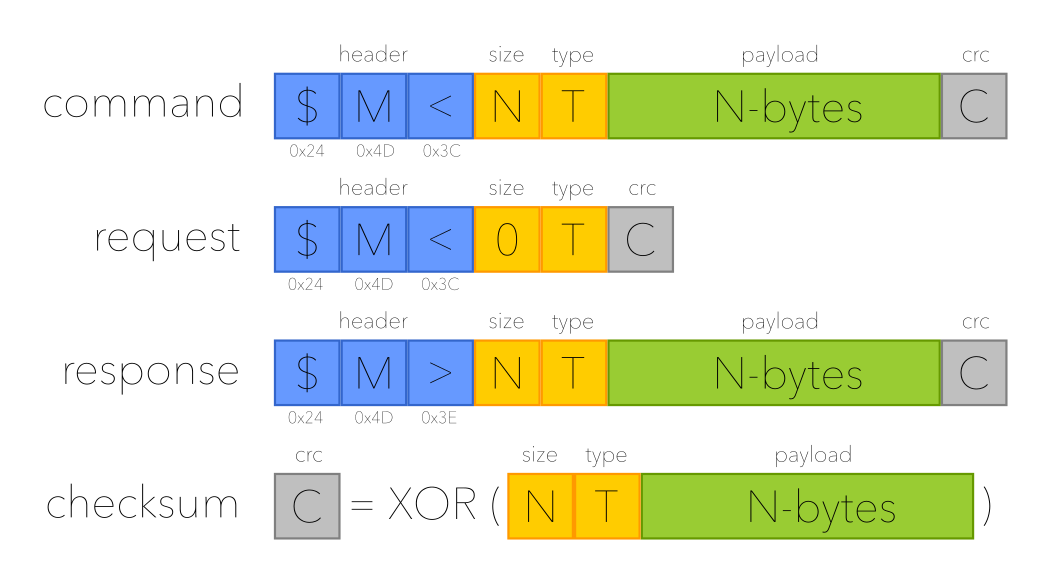
\includegraphics[width=0.9\textwidth]{images/msp_frame}
\caption{MultiWii Serial Protocol (MSP) frame format}
\label{fig:msp}
\end{figure}

In MSP, frames can always be sent to the flight controller (quadcopter). But, in order to receive frames from the flight controller, one has to send a request frame to the flight controller. The request frame is very similar to a command frame, except that its data length is zero and consequently, the checksum is just the MSP code.\\

\section{Control Algorithm}
The control algorithm plays a vital role in the stabilization quadcopter. The entire functionality implemented in the firmware until this point serves as the input to the control algorithm, to debug/visualize the data for designing the control architecture and finally to transfer the output of the control algorithm as PWM values to the different motors.\\

The stabilization control basically deals with how much power should be given to each of the motor based on the orientation of the quadcopter. To stabilize the quadcopter in mid-air, it is evident that we have to control the pitch, roll and yaw motion and hence a controller will have to be implemented in each of the axis. Another controller will have to designed to handle the throttle, given by the user to maintain a certain altitude. Another question that arises is how will the four different motors be controlled in order to stabilize. The later will be discussed towards the end of this section.\\

The control architecture chosen in this firmware is a parallel proportional integral derivative (PID) architecture. \textit{\autoref{fig:pid}} shows the block diagram for the same. PID is a sum of three different terms, each of which and their contributions to the output is explained below.\\

\begin{figure}[!htb]
\centering
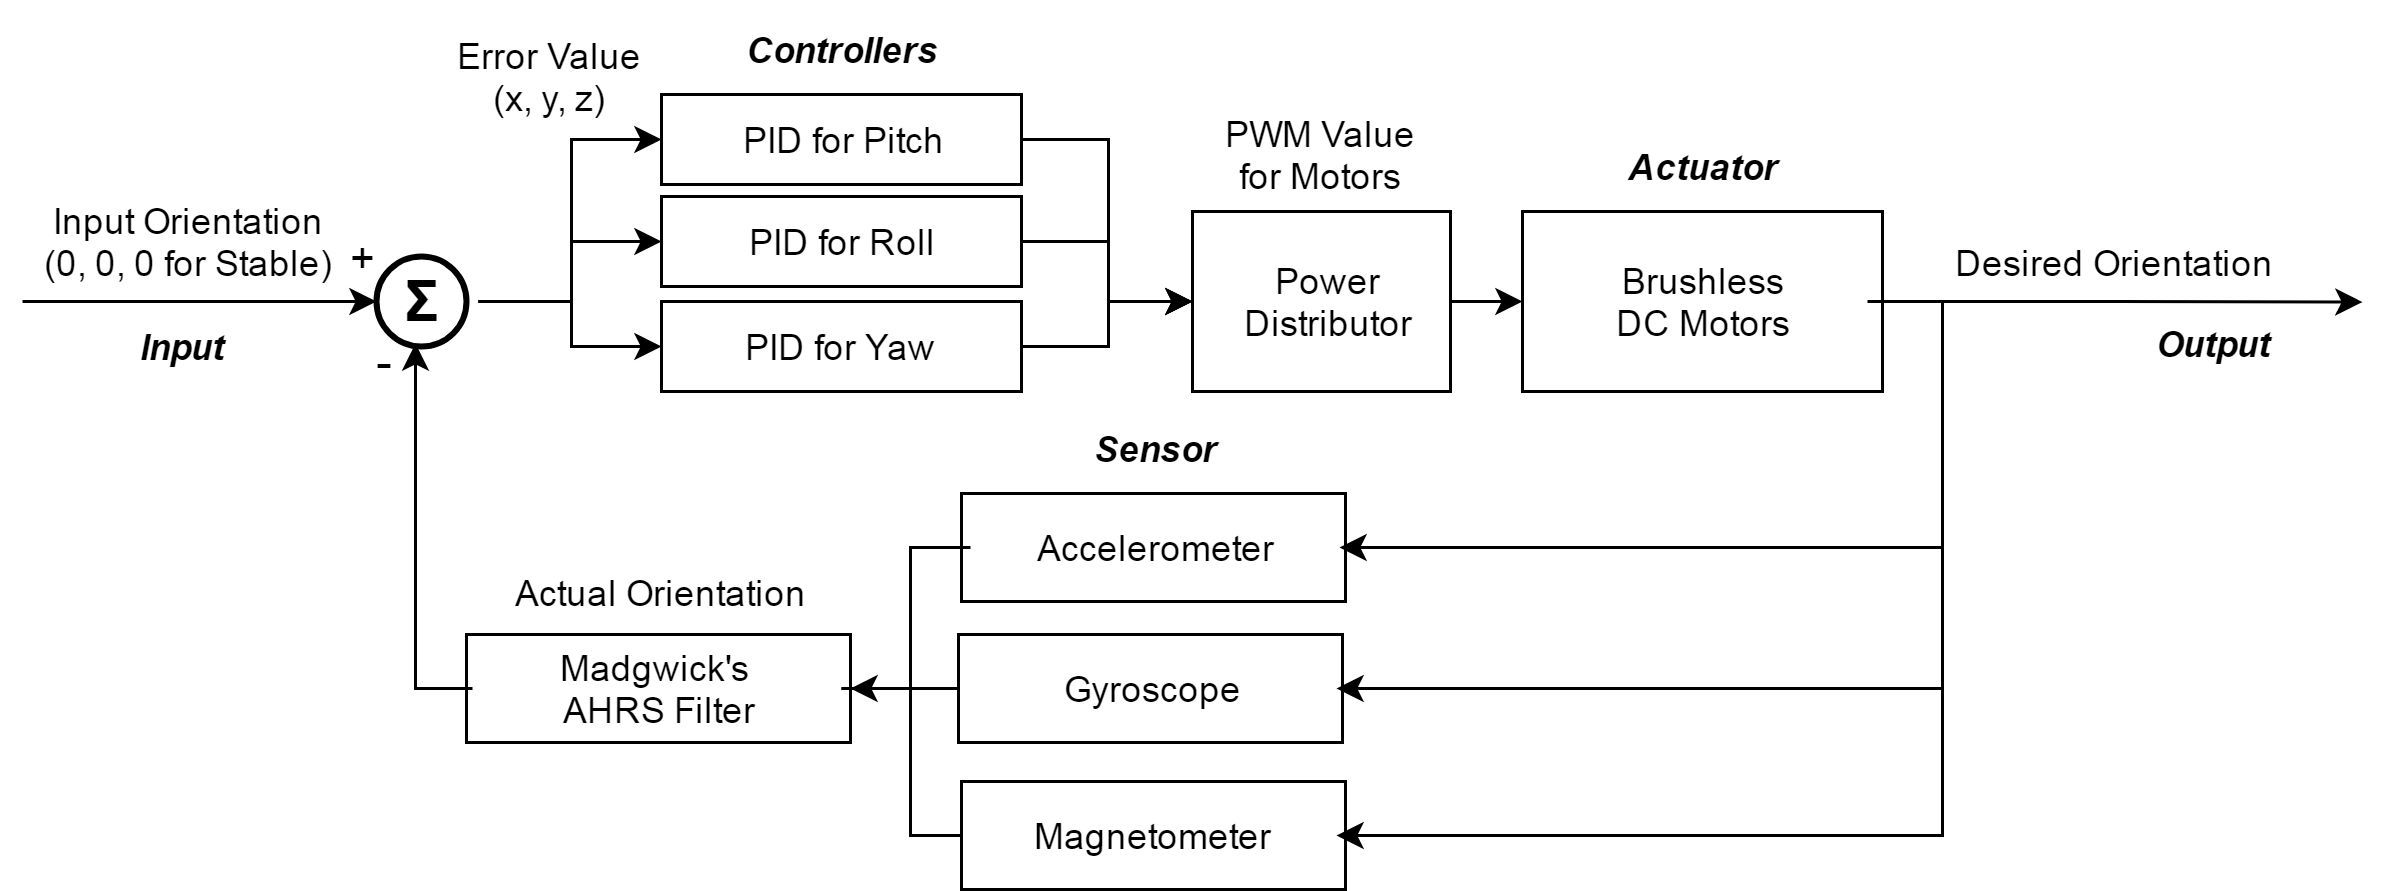
\includegraphics[width=\textwidth]{images/pid}
\caption{Parallel PID architecture for orientation stabilization}
\label{fig:pid}
\end{figure}

\textbf{Proportional Term} | The response of the proportional term is simply a constant (Kp) times the current error. Error is the difference between the desired position (Set Point) and the current position (orientation angle). Higher the magnitude of the error, higher will be its response in the overall PID output in order to minimize the error in the current position. A very low gain (Kp) will make the quadcopter very unresponsive. Whereas, a high gain will make the quadcopter over responsive. The controller will not only correct the present error but will also introduce its own error, and in turn tries the correct this self-induced error again. Hence, it induces oscillations about the desired position. As oscillations become larger and larger, the quadcopter will became unstable and finally crash. It is evident that a steady state error always persists. Response of the proportional term is given below. 

\begin{center}
\begin{BVerbatim}
proportional_term = kp * error
\end{BVerbatim}
\end{center}

\bigskip

\textbf{Integral Term} | The integral term sums up the amount of error over time. This term depends on the present magnitude of error as well as the past errors. The integral term helps in accelerating the current position towards the desired set point. This term will continually contribute to the overall response until the error becomes zero. It tries to eliminate any residual error (steady state) that should have been previously corrected. Higher the magnitude of the error, faster will be the response to minimize it. However, since it keeps accumulating errors over time and accelerates towards the set point, an overshoot will occur before it reaches the desired set point. Another problem is the wind-up phenomenon, which occurs when the accumulated error is beyond the maximum actuator output and can be solved by limiting its response in the output. The response of the integral term is given below.

\begin{center}
\begin{BVerbatim}
integral_sum += (error * sampleTime)
integral_term = ki * constrain(integral_sum, -LIMIT, +LIMIT)
\end{BVerbatim}
\end{center}

\bigskip

\textbf{Derivative Term} | The derivative term is proportional to rate of change of error. It is not dependent on the current magnitude of error and is incapable of minimizing the error on its own. The purpose of the derivative term is to anticipate the future behavior of the error. Thus, it helps in achieving the desired position much faster and reduces the unwanted overshoot caused by the integral term. The derivative term helps in damping the oscillations. However, a high magnitude of derivative gain (Kd) can induces vibrations in the quadcopter because it amplifies the noise in the system. Derivate response is given below.

\begin{center}
\begin{BVerbatim}
derivative_term = kd * (current_error – previuos_error)/sampleTime
\end{BVerbatim}
\end{center}

\bigskip

Finally, the desired output response can be achieved by tuning these PID gains properly to control their individual contributions in the output. The output of the PID control algorithm is given below.

\begin{center}
\begin{BVerbatim}
PID_output = proportional_term + integral_term + derivative_term
\end{BVerbatim}
\end{center}

\bigskip

\section{Motor Operation}
The \textit{Pluto Drone} and the firmware supports upto six motors. Currently only four motors are used. The motors are coreless motors. Coreless brushed motors have very little inertia because only the coils are connected to the shaft. This is great if you want to abruptly change the speed or the direction of rotation. Coreless motors achieve high RPMs, but very little torque. Torque here is not a very serious issue as the payload of the drone is very less (\SI{60}{\gram}).\\ 

The motor speed control is achieved using \textit{Pulse Width Modulation (PWM)}. As the duty cycle of the pulse width increases, more power is delivered to the motors in a single cycle and as a result they operate at higher speeds. The PWM values range from 0 (stopped) to 1000 (full speed).\\

Essentially when propellers rotate, applying the rotational analog of Newton’s third law of motion, it generates a torque effect on the quadcopter’s body in the opposite direction. Hence, if all motors rotate in the same direction, then the quadcopter will keep rotating (or yaw) in that direction. The cause and effect is an important function to understand with quadcopter blade rotation. In order to counteract this torque effect, we need an equal amount of motors that spin in the opposite direction. \textit{\autoref{fig:quad_blades}} show the motor configurations. \href{http://www.droneybee.com/quadcopter-blade-rotation-lift/}{Here} is a good article to understand the dynamics of a quadcopter.\cite{kada}\\

\begin{figure}[!htb]
\centering
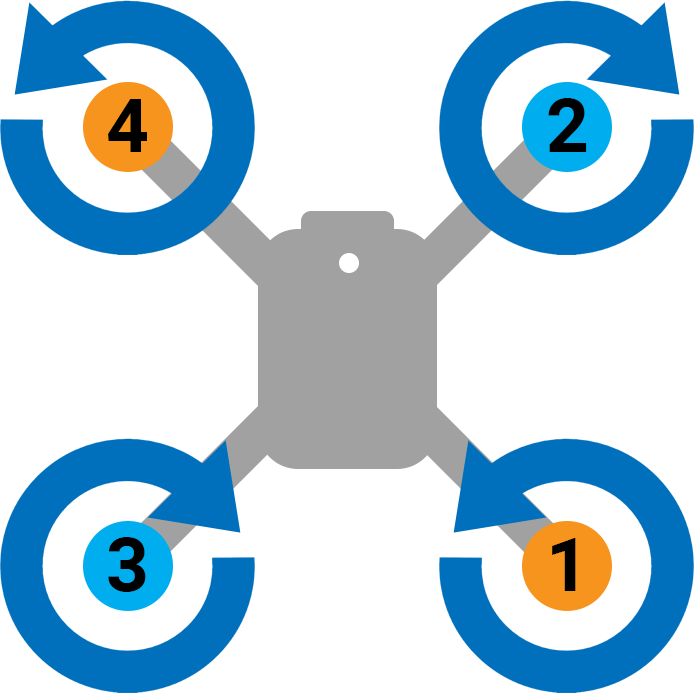
\includegraphics[width=0.45\textwidth]{images/quad_basic}
\caption{Clockwise and Anti-clockwise motor configuration for a quadcopter}
\label{fig:quad_blades}
\end{figure}

The next step is distribute the PID output to the different motors of the quadcopter. The power distribution is much simpler to implement than described in theory. Consider the quadcopter in \textit{\autoref{fig:quad_blades}} with four motor labeled M1 to M4. If the quadcopter experiences a tilt in the forward direction (the pitch axis), motors M2 and M4 will have to provide more thrust in order to bring the copter back to stable level.\\

Thus the pitch PID output value will be added to the front set of motors (M4 and M2) and be subtracted the back set of motors (M1 and M3). In case there a tilt in the backward direction, here the error will negative and the same distribution algorithm will work. \textit{\autoref{fig:pitch}} shows a representation of the same.\\

\begin{figure}[!htb]
\centering
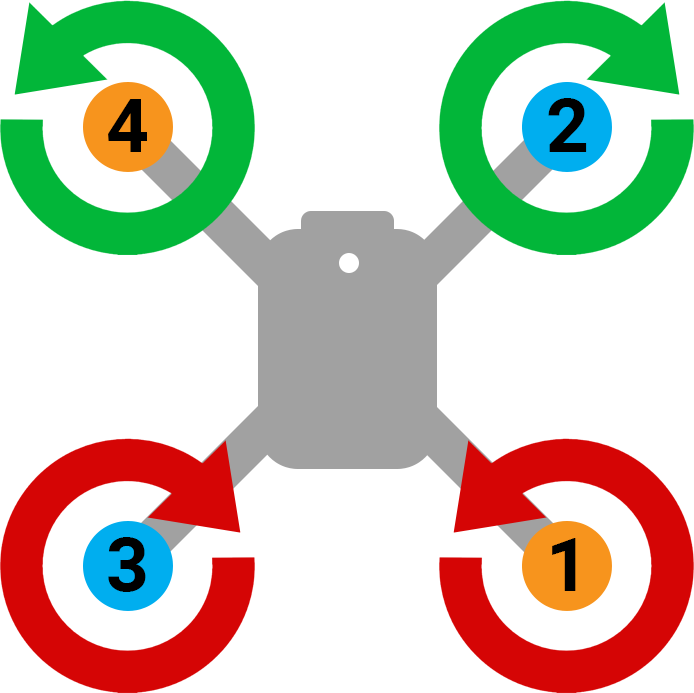
\includegraphics[width=0.35\textwidth]{images/pitch}
\caption{Pitch axis control (Red:0 - Green:1000)}
\label{fig:pitch}
\end{figure}

Stabilization of the roll axis works in a similar way. But, here the tilt correction takes place in the left-right direction. Therefore, roll PID output will have to subtracted from the left set of motors (M3 and M4) and added to the right set of motors (M1 and M2) as shown in \textit{\autoref{fig:roll}}.\\

\begin{figure}[!htb]
\centering
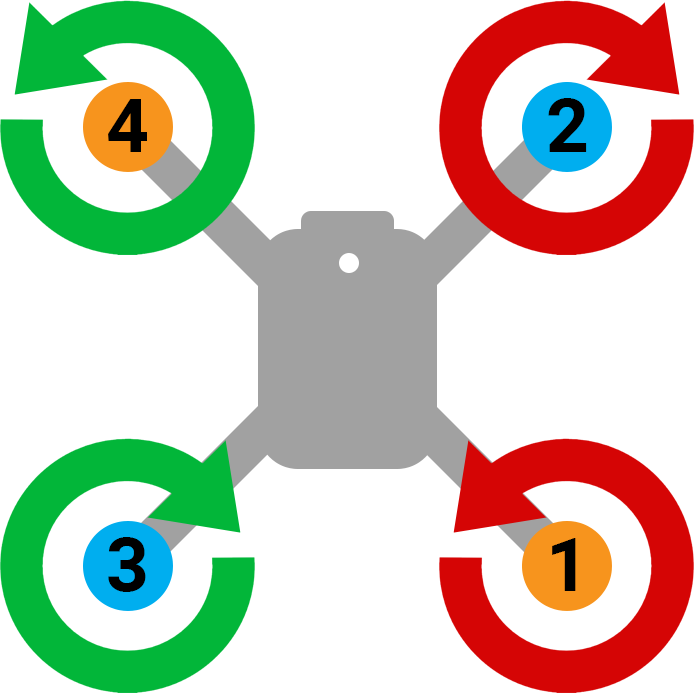
\includegraphics[width=0.35\textwidth]{images/roll}
\caption{Roll axis control (Red:0 - Green:1000)}
\label{fig:roll}
\end{figure}

For yaw stabilization, diagonally opposite motors will have to provide more thrust to bring about a rotational torque and hence change the yaw as shown in \textit{\autoref{fig:yaw}}.\\

\begin{figure}[!htb]
\centering
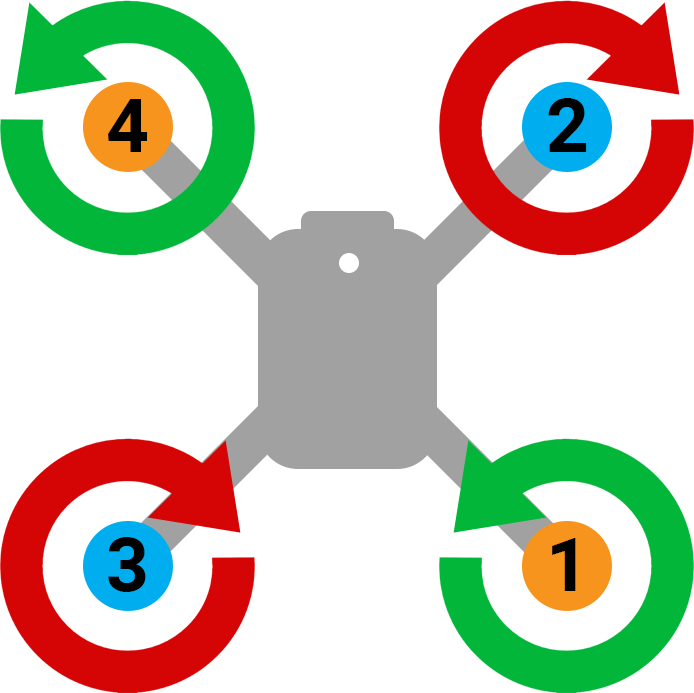
\includegraphics[width=0.35\textwidth]{images/yaw}
\caption{Yaw axis control (Red:0 - Green:1000)}
\label{fig:yaw}
\end{figure}

Summing up all the outputs from the different axes, the following motor distribution algorithm can be obtained. An equal amount of thrust given to all motors varies the altitude of the drone.\\

\begin{center}
\begin{BVerbatim}
M1 = throttle - pitch + roll + yaw  // Back Right
M2 = throttle + pitch + roll - yaw  // Front Right
M3 = throttle - pitch - roll - yaw  // Back Left
M4 = throttle + pitch - roll + yaw  // Front Left	
\end{BVerbatim}
\end{center}

\bigskip

\section{Wireless Joystick Controller}
A very common method of piloting drones is by using a RC transmitter with 6-8 channels. In this project an USB-HID gamepad controller is interfaced with Python, which in turn transmits commands (MSP frames) to the quadcopter over Wi-Fi. Other than throttle and direction control for drones, there are certain other controls that must be provided to a pilot for a stable and safe flight. Following is the list of the set of basic controls implemented in the current firmware.\\

\begin{itemize}
\item \textbf{Throttle} | This sets the base throttle value for all the motors in manual control mode and is used to control the altitude set point in auto flight mode.

\item \textbf{Roll} | This channel varies the set point for the roll angle. A change in the roll set point makes the drone move in the left-right direction.

\item \textbf{Pitch} | This channel varies the set point for the pitch angle. A change in the pitch set point makes move in the forward-backward direction.

\item \textbf{Yaw} | This channel varies the set point for the yaw angle. A change in the yaw set point makes the drone rotate either in the clockwise or anti-clockwise direction.

\item \textbf{Arm} | Initially, when the drone in switched on, the motors must be disabled for safety. When the drone is ready for flight, the pilot must enable the motors and this is referred to as Arming the drone.

\item \textbf{Altitude Hold} | This control toggles between manual and auto flight modes. In manual flight mode, the user is responsible for maintaining the altitude by varying the throttle. In auto mode, the drone will hold its current altitude.

\item \textbf{Pitch Trim} | This adds an offset angle to the pitch axis so that drone is perfectly balanced about this axis.

\item \textbf{Roll Trim} | This adds an offset angle to the roll axis so that drone is perfectly balanced about this axis.\\
\end{itemize}
Further details on the usage of the joystick controller in explained in \textit{\autoref{sec:joystick}}.


\chapter[Usage and Demonstration]{Usage and Demonstration}

\section{Firmware Usage}

\section{Wireless Joystick Controller}
\label{sec:joystick}

\section{Results and Demonstration}

Final Setup Image

User Instruction for demonstration

\href{http://www.youtube.com}{Youtube Link} of demonstration video 

\chapter[Future Work]{Future Work}
A flight controller firmware is a very complex one as it has to support various hardware devices and should be designed in a way such that the addition of new hardware or expansion in functionality must be an easy process. For example, if a new module such as GPS or XBee communication is required, such a change must easily be able to be incorporated into the the current firmware.\\

Another aspect of a flight controller firmware is that it should be somewhat more generic and must be able to support constant hardware modifications, especially in this case as flight hardware has a greater probability of incurring damage. From this perspective, following is a list of features that can be integrated into the current firmware in the future.\\

\begin{itemize}
\item \textbf{Altitude Stability} | In the current firmware, the MS5611 barometer is interfaced and estimated altitude is obtained as well. There is also provision made for altitude control in the PID algorithm. However, altitude hold and stability is still not complete. Ranging sensor such as a LASER sensor or Ultrasonic sensor can be fused with the barometer data to obtain a better estimate of the altitude.\\

\item \textbf{Control Algorithm} | Currently, the motors need to be well calibrated so that each of them provide roughly an equal amount of thrust. So either by fine  tuning the PID gains or re-implementing the control algorithm, achieving stable flight for any get set of motors is a task.\\

\item \textbf{Auto Sensor Calibration} | Auto calibration of sensors, the gyroscope and magnetometer in particular, is another feature that can in built within the firmware itself. Currently, sensor calibration is performed externally by sending data samples to a Python script.

\item \textbf{Localization} | The current firmware has no support for localization. Adding features such as GPS for outdoor way-point navigation and return-to-home feature would be very helpful. The MSP currently implemented already supports the addition of GPS module.\\

\item \textbf{Safe Landing Feature} | The flight dynamics vary a lot when the battery level is low. In fact, the micro-controller begins to reboot several times due to insufficient power when all the motors are on. Interfacing the battery monitoring sensor (already present on-board) and implementing a safe landing feature once the voltage level drops below a certain voltage should be integrated with the firmware.\\

\item \textbf{Error Handling} | There are several sources of error that may occur in the firmware such as I2C errors, UART errors and so on. Currently if an error occurs, the program control transfers into a while loop and prints the file name and line number on the serial terminal, at where the error had occurred. To make the firmware more robust and safe, better error handling can be implemented.\\  

\item \textbf{Custom Joystick Controller} | In this project, a XBOX One USB-HID gamepad controller is used. In the future a custom wireless controller can be developed from scratch using the ESP8266 Wi-Fi module.

\end{itemize}

\chapter[Bug Report and Challenges]{Bug Report and Challenges}
Any issues in code and hardware.

Any failure or challenges faced during project

%-------------------------------------------------------------------


\begin{thebibliography}{20}
\addcontentsline{toc}{chapter}{References}

\bibitem{geob}
Geoffrey Brown,
\href{https://www.cs.indiana.edu/~geobrown/book.pdf}{\textit{Discovering the STM32 Microcontrollers}}, 2016.

\bibitem{stm32}
STMicroelectronics, \href{http://www.st.com/content/st_com/en/products/microcontrollers/stm32-32-bit-arm-cortex-mcus/stm32f1-series/stm32f103/stm32f103rb.html}{\textit{Mainstream Performance line, ARM Cortex-M3 MCU}}.

\bibitem{gnu}
ARM Developer, \href{https://developer.arm.com/open-source/gnu-toolchain/gnu-rm}{\textit{GNU ARM Embedded Toolchain}}.

\bibitem{stm32hal}
STMicroelectronics, \href{./datasheets/STM32F1 HAL Manual.pdf}{\textit{STM32F1xx HAL Manual}}

\bibitem{carmine}
Carmine Noviello, \href{http://www.carminenoviello.com/2014/12/28/setting-gcceclipse-toolchain-stm32nucleo-part-1/}{\textit{Setting up a GCC/Eclipse toolchain for STM32Nucleo - Part 1}}

\bibitem{ahrswiki}
Wikipedia Article, \href{https://en.wikipedia.org/wiki/Attitude_and_heading_reference_system}{\textit{Attitude and heading reference system}}

\bibitem{ardu}
Arducopter, \href{http://www.arducopter.co.uk/all-arducopter-guides/arducopter-flight-modes}{\textit{
Arducopter Flight Modes}}, 2013

\bibitem{mpu9250}
InvenSense, \href{https://www.invensense.com/products/motion-tracking/9-axis/mpu-9250/}{\textit{MPU-9250 Nine-Axis (Gyro + Accelerometer + Compass) MEMS MotionTracking™ Device}}

\bibitem{tonik}
Toni Corinne, \href{https://www.sparkfun.com/users/194976}{\textit{Accelerometer Basics}} at SparkFun

\bibitem{gyro}
A1ronzo, \href{https://learn.sparkfun.com/tutorials/gyroscope/how-a-gyro-works}{\textit{Gyroscope}} at SparkFun

\bibitem{kris}
Kris Winer, \href{https://github.com/kriswiner/MPU6050/wiki/Simple-and-Effective-Magnetometer-Calibration}{\textit{Simple and Effective Magnetometer Calibration}}

\bibitem{madgwick}
Sebastian O.H. Madgwick, \href{./datasheets/Madgwick Internal Report.pdf}{\textit{An efficient orientation filter for inertial and inertial/magnetic sensor arrays}}

\bibitem{kada}
V. Kadamatt, \href{http://www.droneybee.com/quadcopter-blade-rotation-lift/}{\textit{Quadcopter blade rotation and lift : How and why}}

\bibitem{fifo}
Simply Embedded, \href{http://www.simplyembedded.org/tutorials/interrupt-free-ring-buffer/}{\textit{UART Receive Buffering}}

%\bibitem{},\href{}{\textit{}}
%\bibitem{},\href{}{\textit{}}
%\bibitem{},\href{}{\textit{}}

\end{thebibliography}

%-------------------------------------------------------------------

\chapter*[]{Appendix A: Circular Buffer}
\addcontentsline{toc}{chapter}{Appendix A: Circular Buffer}

\end{document}

